\chapter{印刷}

 B 演習室には、 5 台のプリンタがある。
これらのプリンタは、ネットワークにつながっていて、ネットワークを使って
それぞれのマシンから印刷することができる。

プリンタはすべて PostScript の白黒プリンタで、
 PostScript 形式のファイルを送ると印刷することができる。

この章では、テキスト・ファイルの PostScript への変換や、印刷方法
などについて紹介する。

\section{テキスト・ファイルの PostScript への変換: \texttt{a2ps-j}}

 B 演習室のプリンタは、 PostScript プリンタで、
ファイルを印刷するには、 PostScript 形式に変換する必要がある。

 \texttt{a2ps-j} というコマンドを使うと、テキスト・ファイルを PostScript 形式
に変換することができる。

例えば、「\texttt{renshuu1}」というテキスト・ファイルから、「\texttt{renshuu1.ps}」という
 PostScript 形式のファイルを作るには、次のようにする。

\begin{progls}
% \slbfl{a2ps-j renshuu1 \TG renshuu1.ps}
\end{progls}

\texttt{ls} で確認してみよう。
確かに「\texttt{renshuu1.ps}」ができていることが確認できると思う。
このようにして変換した PostScript ファイルは、
 1 枚に 2 ページ分が横向きに印刷される。

\begin{figure}[H]
\centering{\includegraphics[scale=0.25]{unix14-2.eps}}
\end{figure}

\newpage

もしも、大きめに 1 枚に 1 ページ分を印刷したい場合には、
次のようにして PostScript ファイルを作る。

\begin{progls}
% \slbfl{a2ps-j -p renshuu1 \TG renshuu1.ps}
\end{progls}

\begin{figure}[H]
\centering{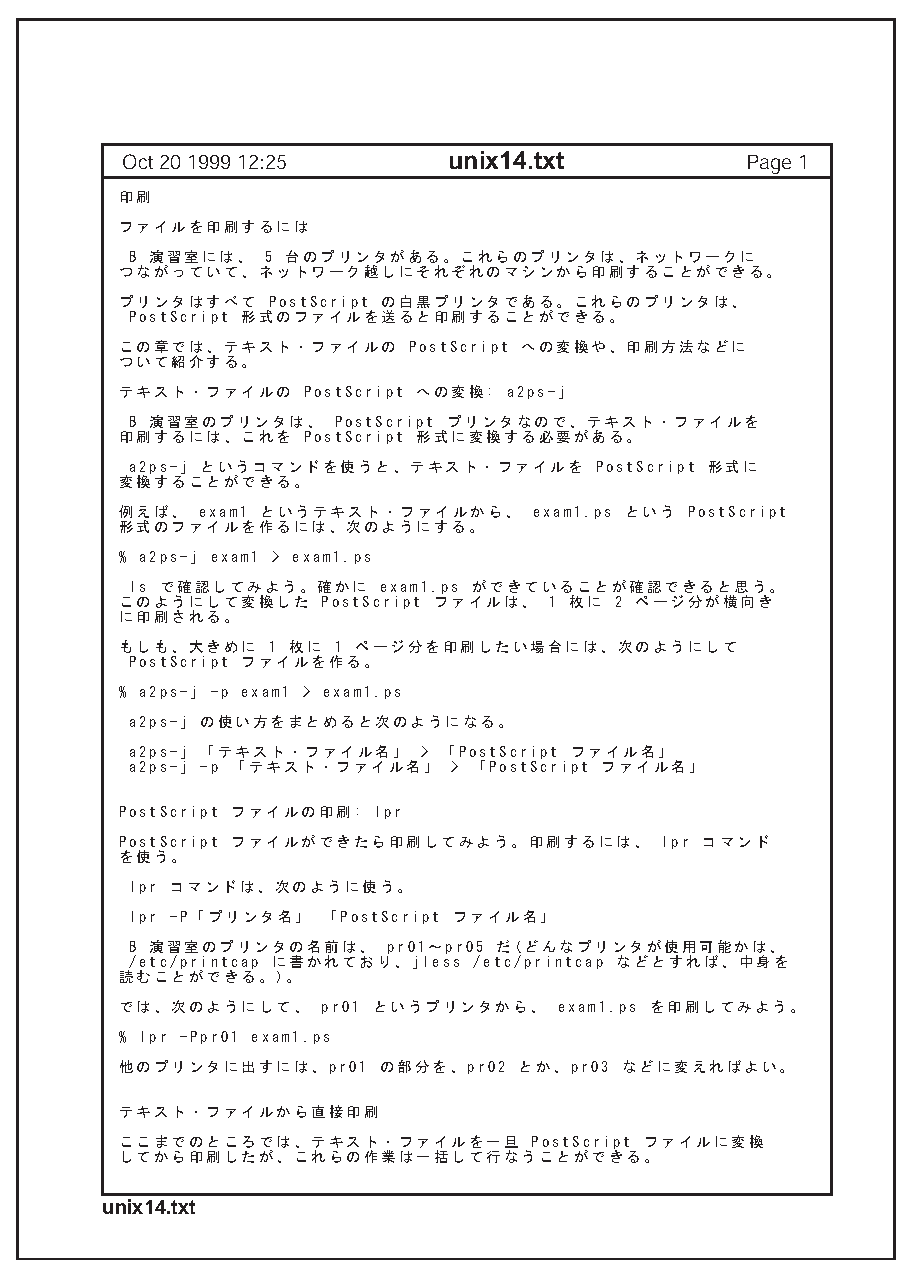
\includegraphics[scale=0.35]{unix14p-2.eps}}
\end{figure}

 \texttt{a2ps-j} の使い方をまとめると次のようになる。

\begin{coml}{16cm}
{\normalsize 1 枚に 2 ページ分印刷したいとき}\\
\texttt{a2ps-j} 「テキスト・ファイル名」 \TG 「PostScript ファイル名」
\end{coml}

\begin{coml}{16cm}
{\normalsize 1 枚に 1 ページ分印刷したいとき}\\
\texttt{a2ps-j -p} 「テキスト・ファイル名」 \TG 「PostScript ファイル名」
\end{coml}

%\newpage

\section{PostScript ファイルの印刷: \texttt{lpr}}

PostScript ファイルができたら印刷してみよう。
印刷するには、次のようにして \texttt{lpr} コマンドを使う。

\begin{coml}{12cm}
\texttt{lpr -P}「プリンタ名」 「PostScript ファイル名」
\smallskip
\end{coml}

なお B 演習室のプリンタの名前は、 \texttt{pr01}〜\texttt{pr05} である
\footnote{どんなプリンタが使用可能かは、 \texttt{/etc/printcap} に書かれており、
 \texttt{jless /etc/printcap} などとすれば、中身を読むことができる。}。

では、次のようにして、 \texttt{pr01} というプリンタから、
「\texttt{renshuu1.ps}」を印刷してみよう。

\begin{progls}
% \slbfl{lpr -Ppr01 renshuu1.ps}
\end{progls}

他のプリンタに出すには、 \texttt{pr01} の部分を、 \texttt{pr02} とか、
 \texttt{pr03}、・・・などと変えればよい。

\section{テキスト・ファイルから直接印刷}

ここまでのところでは、テキスト・ファイルを一旦 PostScript ファイルに
変換してから印刷したが、これらの作業は一括して行なうことができる。

具体的には、次のようにする。

\begin{progls}
% \slbfl{a2ps-j renshuu1 \PIPE lpr -Ppr01}
\end{progls}

このように「\texttt{|}」を用いると、 2 つのコマンドをまとめて一括する
ことができる。

\begin{figure}[H]
\centering{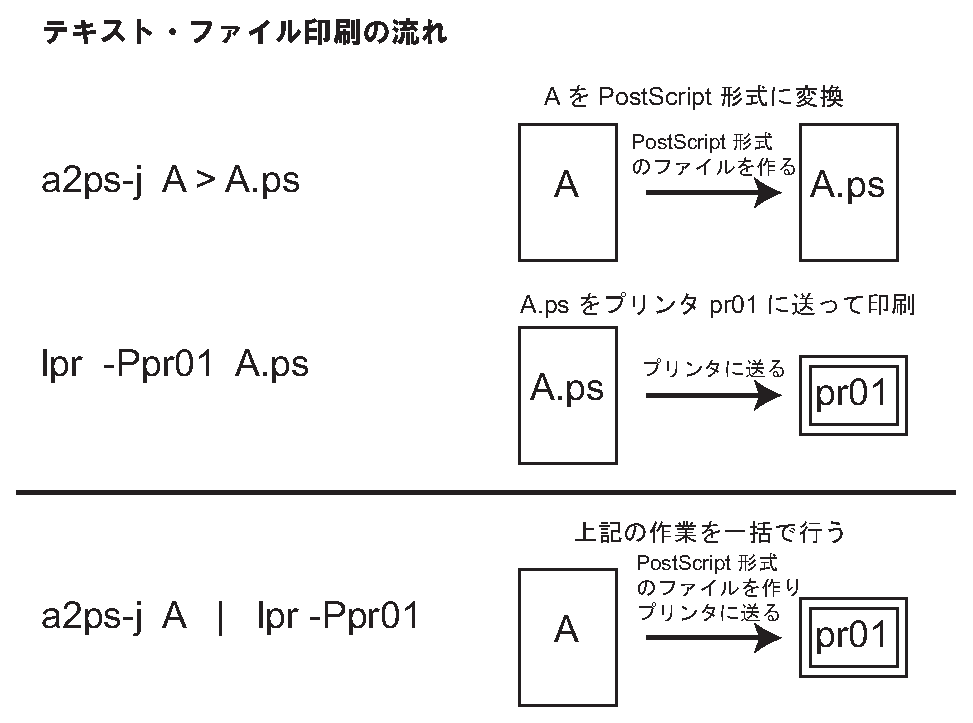
\includegraphics[scale=1.0]{lprflow.eps}}
\end{figure}

\newpage

\section{印刷状況の確認と取消: \texttt{lpq} と \texttt{lprm}}

ほとんどの場合、印刷は高速に行なわれるため、
現実には取り消すことは不可能な場合が多いだろう。
しかし、長い文章を印刷したり、紙がつまったりして、印刷状況を確認したり、
印刷を取り消したくなる場合もある。

\subsection{印刷状況の確認: \texttt{lpq}}

現在の印刷状況を確認するには、 \texttt{lpq} を使う。
使い方は、次のようになる。

\begin{coml}{6cm}
\texttt{lpq -P}「プリンタ名」
\end{coml}

たとえば、プリンタ \texttt{pr01} の印刷状況を調べたい場合には、
次のようにすればいい。

\begin{progls}
% \slbfl{lpq -Ppr01}
pcux48.edu3.aomori-u.ac.jp: sending to edu3pr05
Rank   Owner      Job  Files                                 Total Size
1st    ei00000    259  renshuu1.ps                           22719 bytes
2nd    ei00000    260  (standard input)                      792049 bytes

no entries
\end{progls}

このとき表示されるものの意味は以下の通りである。

\hspace*{5mm}
\begin{minipage}{10cm}
\begin{table}[H]
\renewcommand{\arraystretch}{1.2}
\begin{tabular}{ll}
\textbf{Rank} & 印刷の順番\\
\textbf{Owner} & 印刷を実行しているユーザ\\
\textbf{Job} & 印刷ジョブの番号\\
\textbf{Files} & ファイル名\\
\textbf{Total Size} & ファイルの大きさ
\end{tabular}
\end{table}
\end{minipage}

\bigskip

なお、「\texttt{a2ps-j renshuu1 \PIPE ~lpr -Ppr01}」のように、
一括で印刷を行なっている場合、
ファイル名は「\texttt{(standard input)}」となる。

\newpage

\subsection{印刷の取り消し: \texttt{lprm}}

印刷を取り消すには、次のようにして \texttt{lprm} を使う。

\begin{coml}{11cm}
\texttt{lprm -P}「プリンタ名」 「印刷ジョブの番号」
\end{coml}

例えば、上の例では、印刷ジョブの番号は「259」である。
これを取り消すには、次のようにすればいい。

\begin{progls}
% \slbfl{lprm -Ppr01 259}
dfA259pcux00.edu3.aomori-u.ac.jp dequeued
cfA259pcux00.edu3.aomori-u.ac.jp dequeued
\end{progls}

これで印刷はキャンセルされる。

\newpage

\section{PostScript ファイルの表示: \texttt{ghostview}}

以降の節は、おまけである。

 PostScript ファイルを画面に表示するには、 \texttt{ghostview} コマンドを
使えばよい。

使い方は、次のようになる。

\begin{coml}{11cm}
\texttt{ghostview} 「PostScript ファイル名」 \&
\end{coml}

では、「\texttt{renshuu1.ps}」を表示してみよう。

\begin{progls}
% \slbfl{ghostview renshuu1.ps \&}
\end{progls}

\begin{figure}[H]
\centering{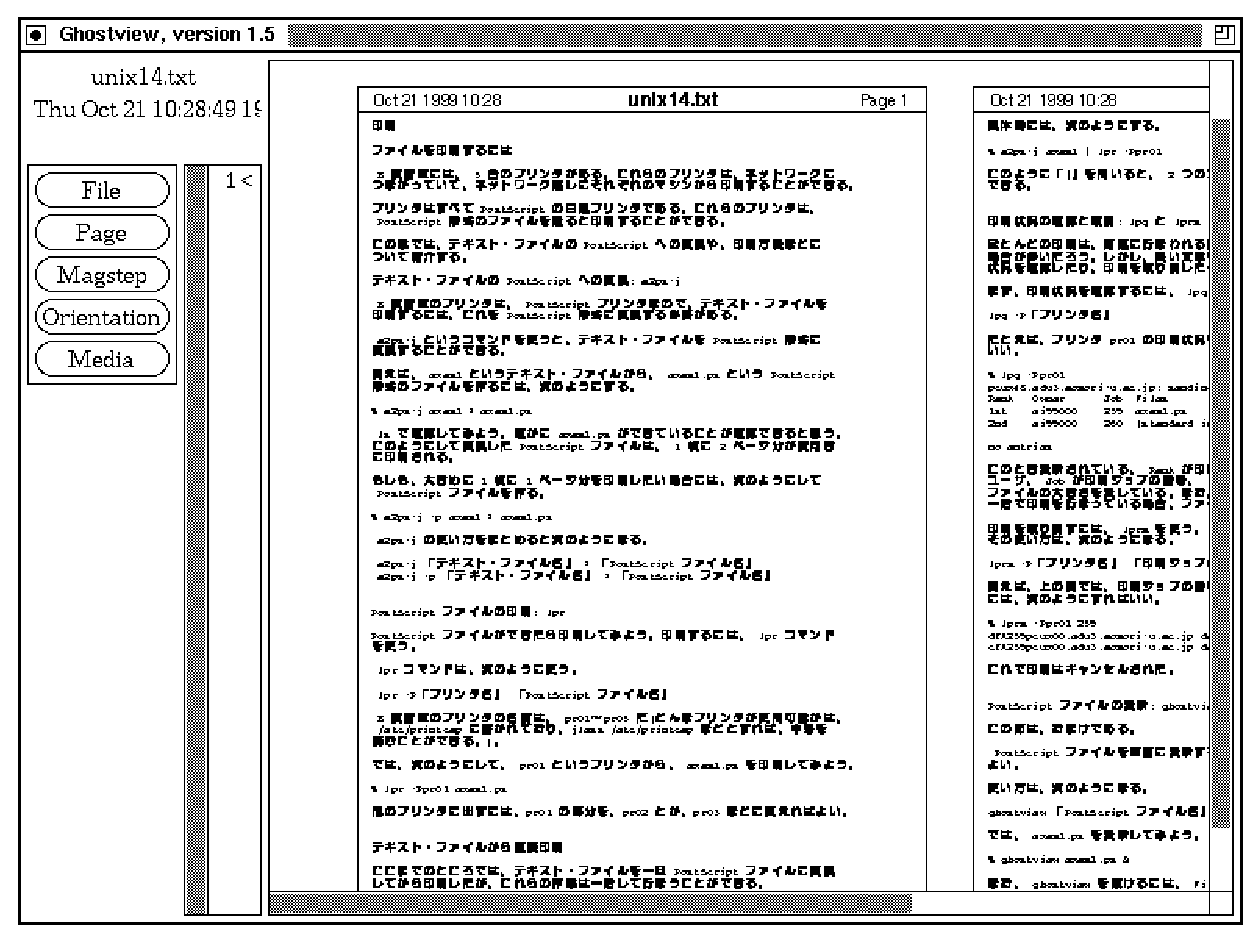
\includegraphics[scale=0.7]{ghostview.eps}}
\end{figure}

なお、 \texttt{ghostview} を抜けるには、 \KEYTOP{File} メニューから、
 \KEYTOP{Quit} を選べばよい。

\newpage

\section{PostScript とはどんなものか?}

 PostScript は、一種のプログラムで、手で書くこともできる。

例えば「\texttt{mule circle.ps \&}」と Mule を起動して、
「\texttt{circle.ps}」というファイルに次のプログラムを入力して保存してみよう。

\setlength{\baselineskip}{5mm}
\begin{center}
\begin{minipage}{32zw}
\begin{itembox}[l]{circle.ps}
\begin{alltt}
%!PS-Adobe-1.0
%%Title: Circle
%%Pages: 1
300 400 100 0 360 arc
stroke
showpage
%%Trailer
\end{alltt}
\end{itembox}
\end{minipage}
\end{center}
\setlength{\baselineskip}{7mm}

これを \texttt{ghostview} で表示したり、 \texttt{lpr} で印刷したりすると、
確かに円が描かれているのがわかると思う。

\begin{figure}[H]
\centering{
\includegraphics[scale=0.25]{circle.eps}}
\end{figure}

このプログラムの意味は別にわからなくてもかまわないが、
一応解説しておこう。
まず、「\texttt{\%}」で始まる行は、コメントである。
それから、「\texttt{300 400 100 0 360 arc}」の部分で、
紙の左上から x 方向に 300 ポイント、 y 方向に 400 ポイントの位置を中心に、
半径 100 ポイント、 0〜360度の範囲の円弧を指定している。
次の「\texttt{stroke}」で線を引くように指定。
そして最後の「\texttt{showpage}」が描画である。

 PostScript は奥がとても深いので、ここできちんとした説明はしない。
ただ、 PostScript プリンタにデータを送るときに、コンピュータはこのような
プログラムに画像データを変換していることは、知っておいて損はない。

\section*{この章で紹介したコマンド}

\begin{center}
\begin{minipage}{13cm}
\begin{itembox}[l]{PostScript への変換と印刷}
\begin{description}
\item[\texttt{a2ps-j} :] テキスト・ファイルを PostScript に変換

使い方: \texttt{a2ps-j} 「テキスト・ファイル名」 \texttt{>} 「PostScript ファイル名」

\hspace*{1cm}大きく印刷するには、 \texttt{-p} オプションを付ける。
\item[\texttt{lpr} :] PostScript ファイルの印刷

使い方: \texttt{lpr -P}「プリンタ名」 「ファイル名」

\hspace*{1cm}なお、 PostScript への変換と印刷を一括で行なうには、

\hspace*{1cm} \texttt{a2ps -j} 「ファイル名」 \texttt{| lpr -P}「プリンタ名」
\item[\texttt{lpq} :] 印刷状況の確認

使い方: \texttt{lpq -P}「プリンタ名」
\item[\texttt{lprm} :] 印刷の取消

使い方: \texttt{lprm -P}「プリンタ名」 「印刷ジョブの番号」
\item[\texttt{ghostview} :] PostScript ファイルの表示

使い方: \texttt{ghostview} 「PostScript ファイル名」 \texttt{\&}
\end{description}
\end{itembox}
\end{minipage}
\end{center}
